%------------------------------------------------------------------------
%Editar Diplomado
\hypertarget{cv:consultarPantalla}{\section{Consultar Pantalla}} \label{sec:consultarPantalla}

	Esta funcionalidad le permitirá consultar la información asociada a una pantalla.

		\subsection{Procedimiento}

			%Pasos de procedimiento
			\begin{enumerate}
	
			\item Oprima el icono \IUConsultar{} de un registro existente de la pantalla \ref{fig:GestionarPantallas} ''Gestionar Pantallas''.
	
			\item Se mostrará la pantalla \ref{fig:consultarPantallaA} ''Consultar Pantalla''.
			
			%Pantalla
			\begin{figure}[htbp!]
				\begin{center}
					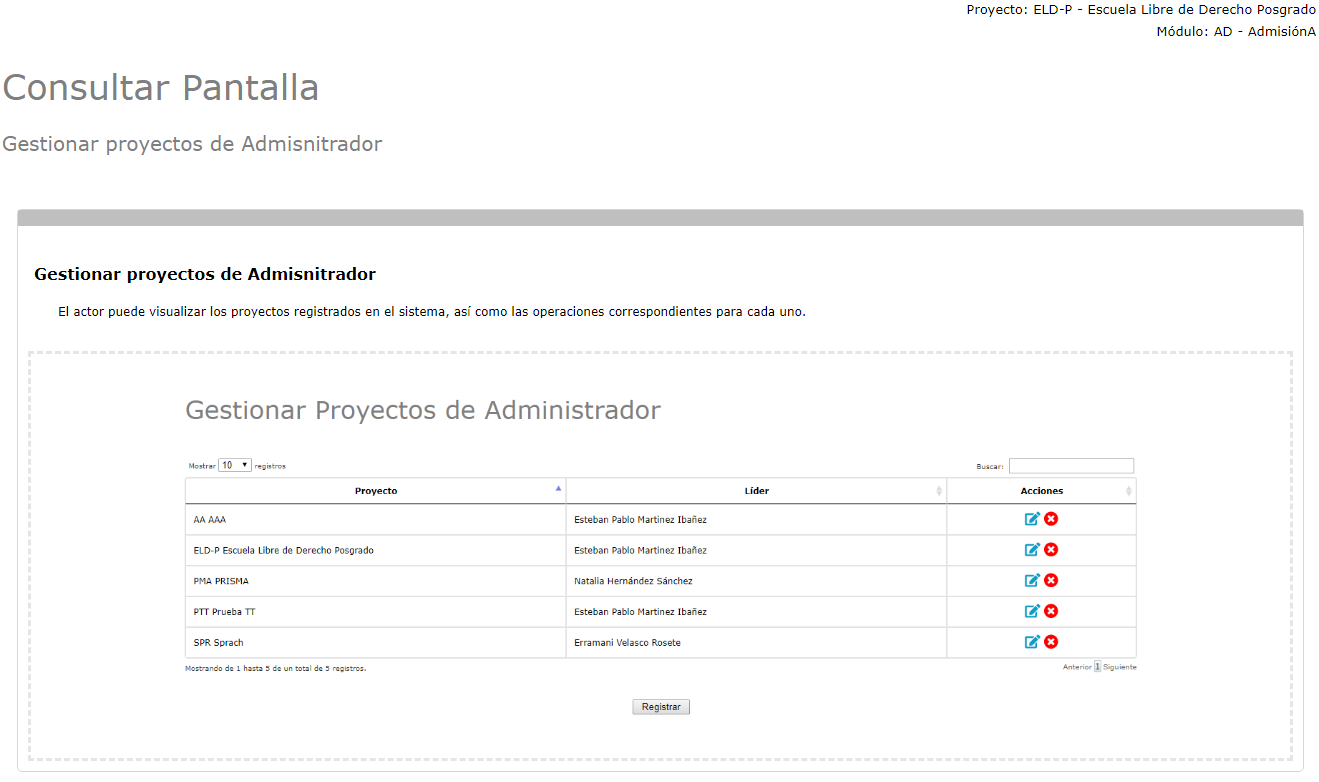
\includegraphics[scale=0.5]{roles/lider/pantallas/pantallas/IU11-4consultarPantallaA}
					\caption{Consultar Pantalla}
					\label{fig:consultarPantallaA}
				\end{center}
			\end{figure}
		
		\begin{figure}[H]
			\begin{center}
				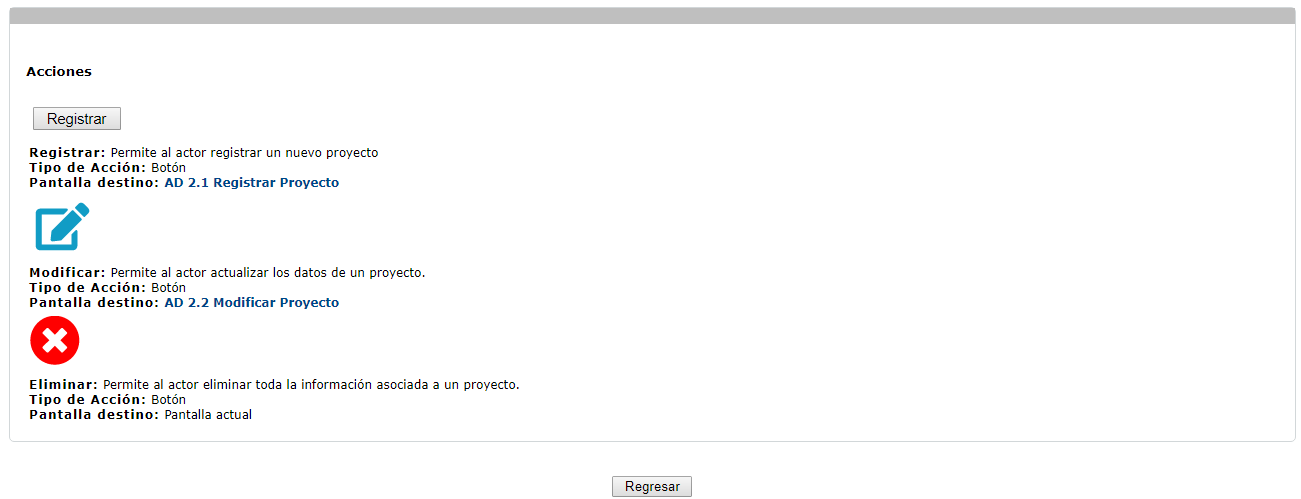
\includegraphics[scale=0.5]{roles/lider/pantallas/pantallas/IU11-4consultarPantallaB}
				\caption{Consultar Pantalla}
				\label{fig:consultarPantallaB}
			\end{center}
		\end{figure}
						
			\item Consulte la información registrada.
			
			\item Oprima el botón \IURegresar.
		\end{enumerate}